\label{sec:Res}
\section*{Results}

\subsection*{Constant environment and density-dependence}

From Sandell et al., we simulated populations. With the introduction of density-dependence, the blablabla...

\textbf{Figure1:} See Fig.~\ref{fig:dd}

Introduction of DD should decrease mean phenotype (lower $s_{0}$) and limit population size

\begin{figure}[ht!]
	\centering
	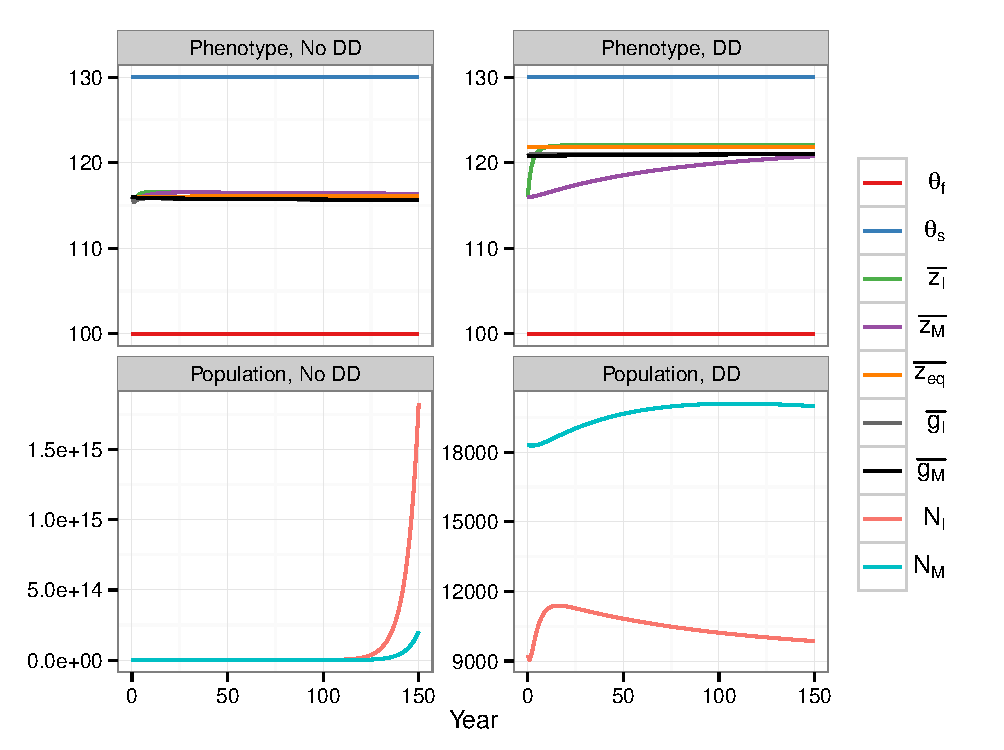
\includegraphics[scale=1]{Figures/DDphenopop.pdf}
	\caption{\textbf{Effect of density-dependence on phenotypes and populations}. Left panel: Phenotype variations in population ($\overline{z_I}, \overline{z_M}$) with their corresponding genotypic values ($\overline{g_I}, \overline{g_M}$) all starting from $z = 166$, and the approximation given by \autoref{eq:zweak}; right panel: demography, number of immature individuals ($N_I$, red), number of mature individuals ($N_M$, blue)} starting from Stable-Stage Distribution (SSD).
	\label{fig:dd}
\end{figure}

\subsection*{Fluctuating optimums}

The noises were drawn from a bivariate normal distribution to make the optimums fluctuate. We varied the correlation between them.

\textbf{Figure2:} See Fig.~\ref{fig:corr}

Explain in the text correlation of $z_{I}$ with $\theta_{s}(t)$

\begin{figure}[ht!]
	\centering
	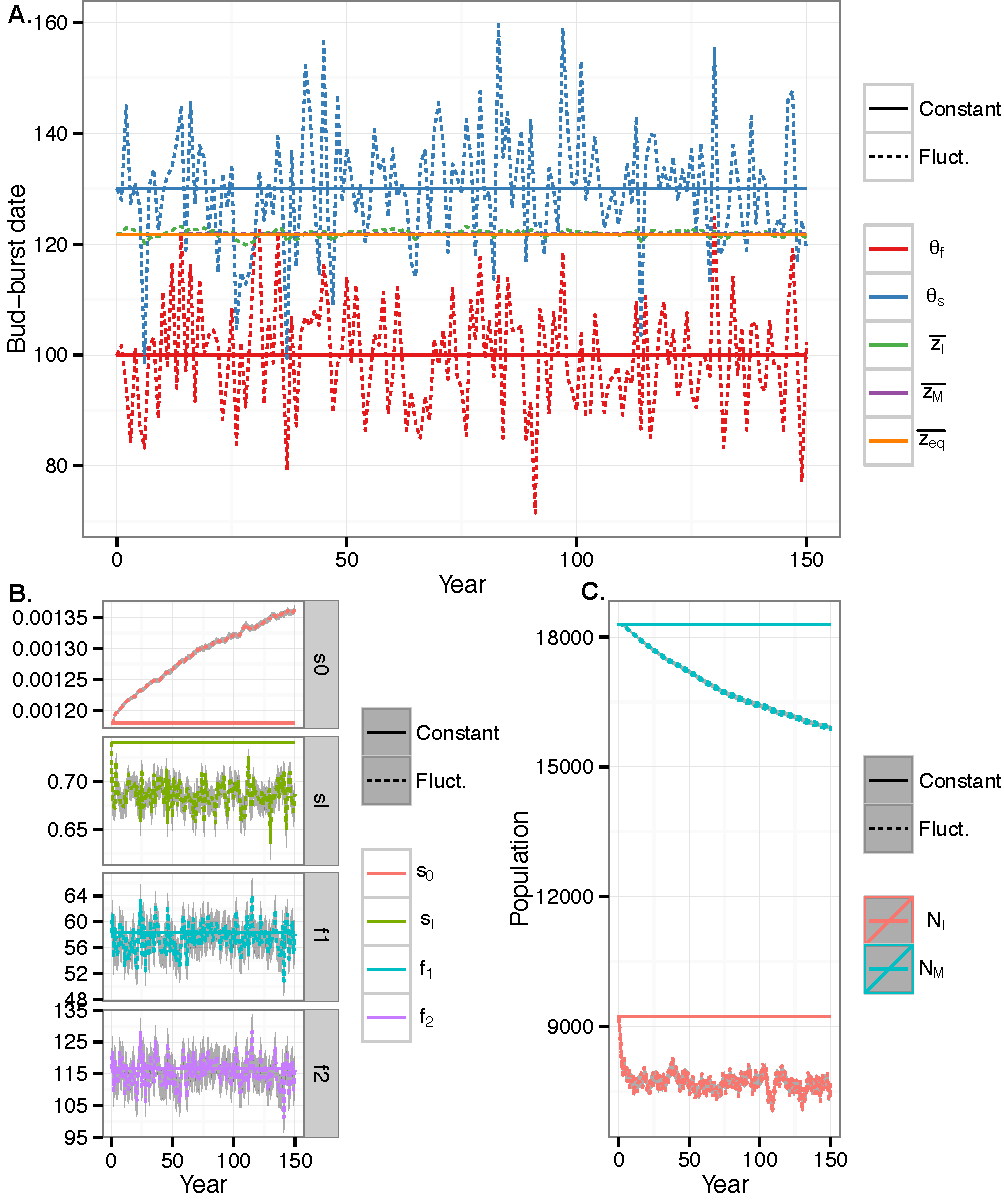
\includegraphics[scale=1]{Figures/PhenoLHTwithCorr.pdf}
	\caption{\textbf{Effect of the correlation of fluctuations on phenotypes and life-history traits}. Correlation coefficient $\rho_{N}$ values of noises are indicated at the the top of each column. Phenotype and approximations are shown in julian days, $\overline{z_\epsilon}$ is the approximation from \autoref{eq:zfluct}. Mean fecundities are in number of seeds produced. The two bottom rows are survival rates, the top one is $\overline{s_I}$ the mean survival of immature individuals, the bottom one is $s_0$ the rate of survival and germination of seeds (see~\nameref{sec:M&M}).}
	\label{fig:corr}
\end{figure}

\subsection*{Trend in the environment}

Decreasing optimums through time to mimic the advance in phenology with climate change.

\textbf{Figure:} Trend 2 panels with and without fluctuations, simulations results phenotype/time (with and without DD)

\subsection*{Estimation of the fluctuations}

\begin{figure}[ht!]
	\centering
	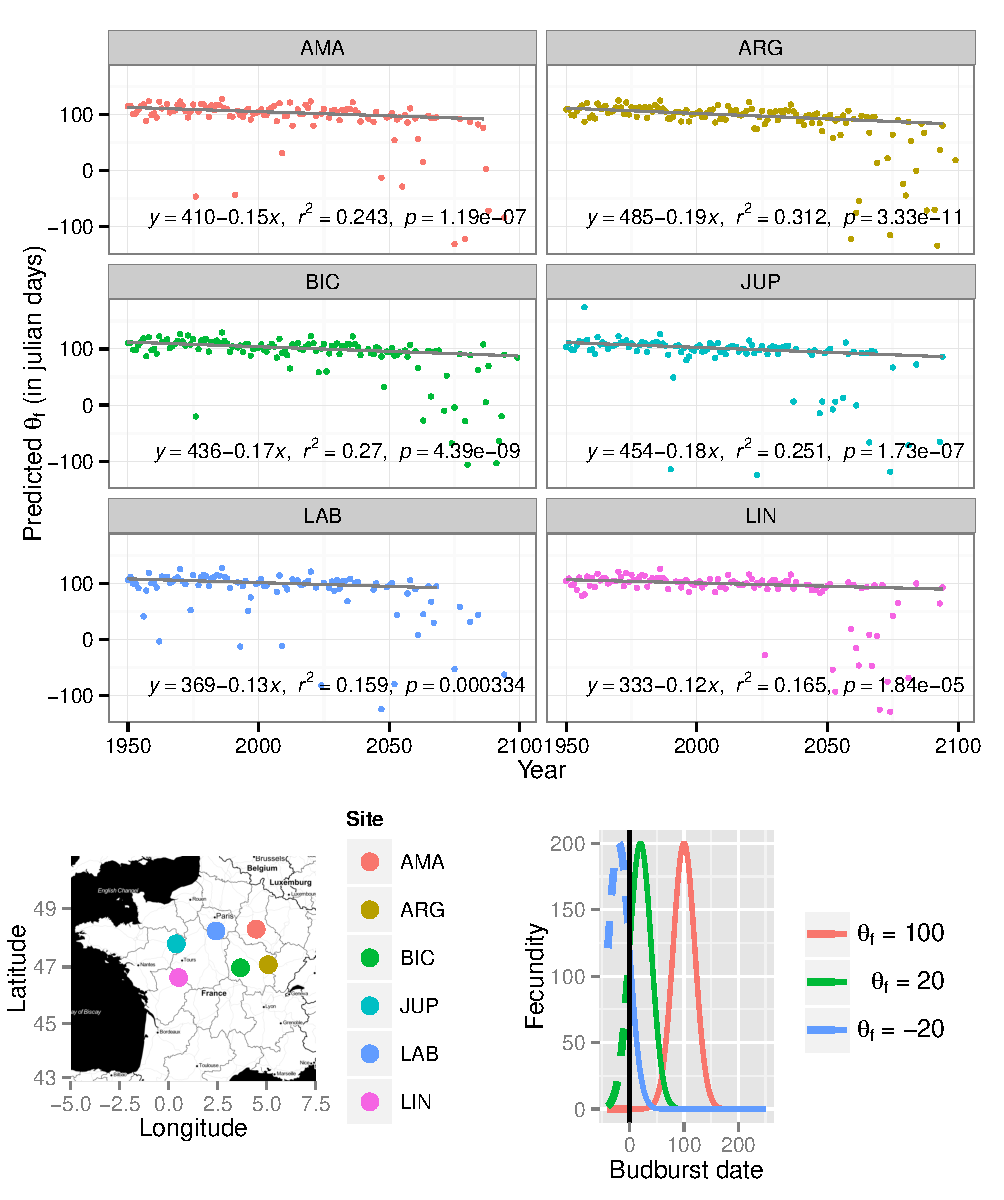
\includegraphics[scale=1]{Figures/optsmaps.pdf}
	\caption{\textbf{$\theta_{f}$ estimations from PHENOFIT data}. Top 3 rows: estimations of $\theta_f$ for each study site see \nameref{sec:M&M} for details. Bottom left panel: map of the study sites. Bottom right panel: Theoretical fecundity functions with parameters from~\autoref{tab:params} with values of $\theta_f$ equals to $100$, $20$ and $-20$, solid lines indicate achievable phenotype, dashed lines show theoretical curves but unreachable phenotypes.}
	\label{fig:thetaf}
\end{figure}

From phenofit.

\textbf{Figure:} Fig.~\ref{fig:thetaf}

\textbf{Table:} table with slope and noise variance estimates for all years, years before 2001 (simulated climate close to real one), after 2001 (projection in climate evolution)